\section{Placement Results}
\label{sec:results}

\end{multicols}

\subsection{Greedy Algorithm (Undirected/Random Moves)}
{
    \centering
    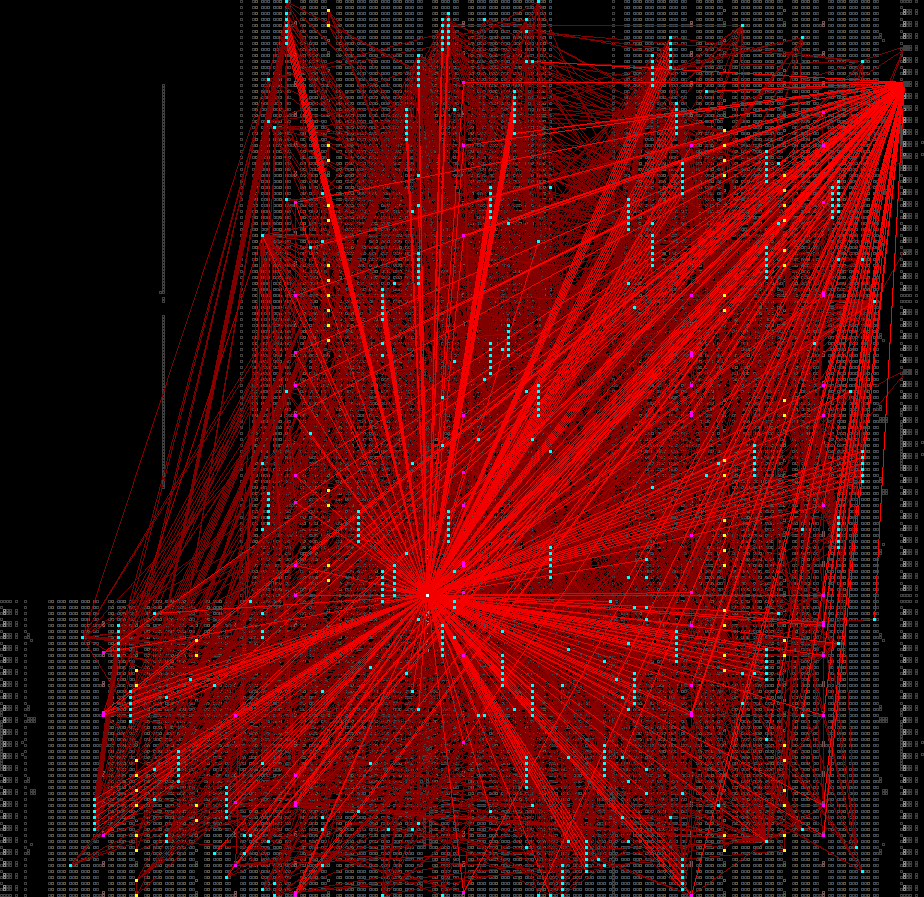
\includegraphics[valign=t, scale=0.25]{figures/results/PlacerGreedyRandom/random_placement.png}
    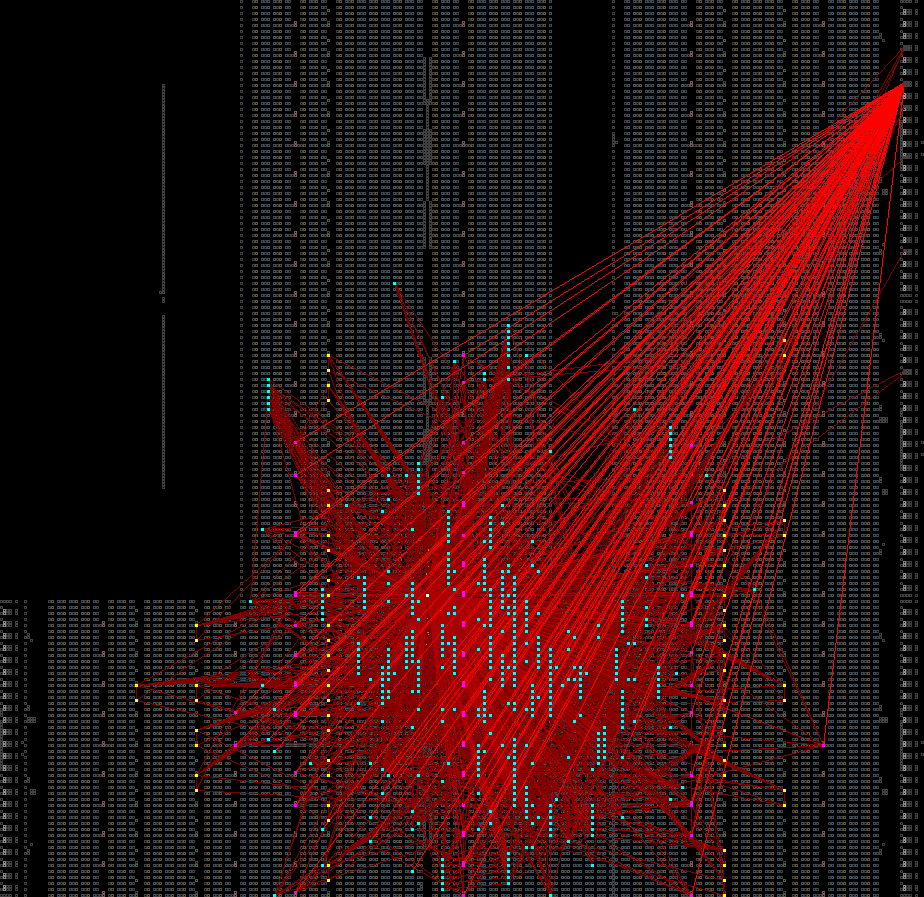
\includegraphics[valign=t, scale=0.25]{figures/results/PlacerGreedyRandom/00000010.png}
    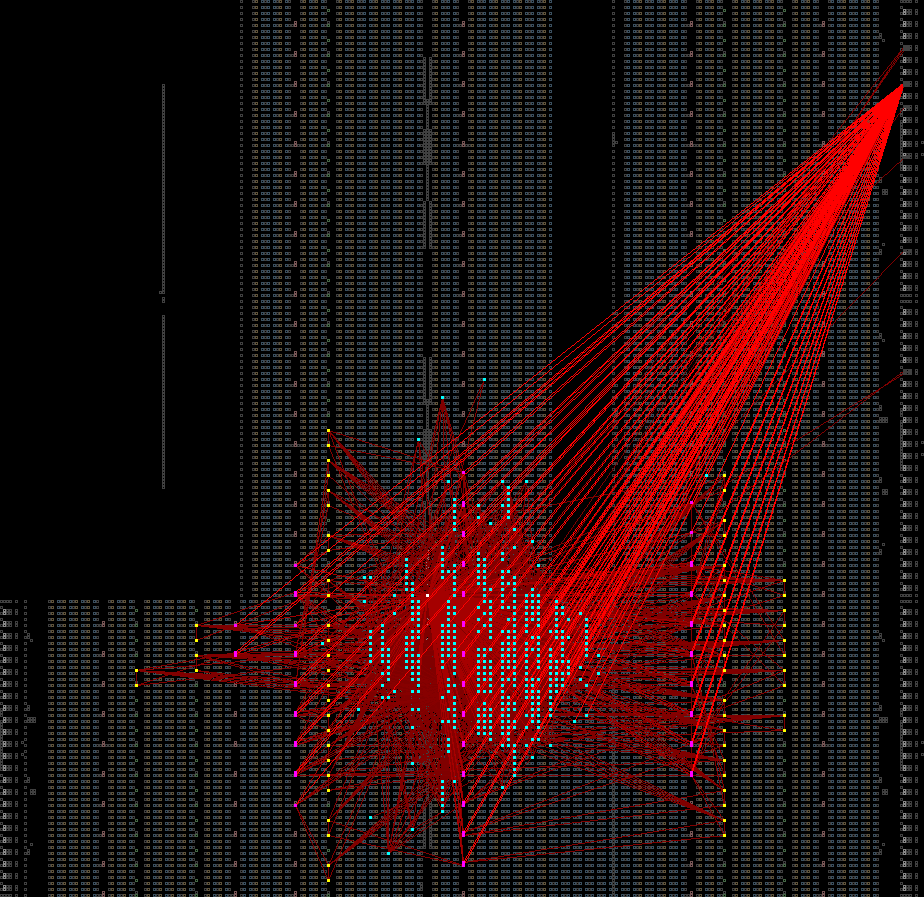
\includegraphics[valign=t, scale=0.25]{figures/results/PlacerGreedyRandom/00000100.png}
    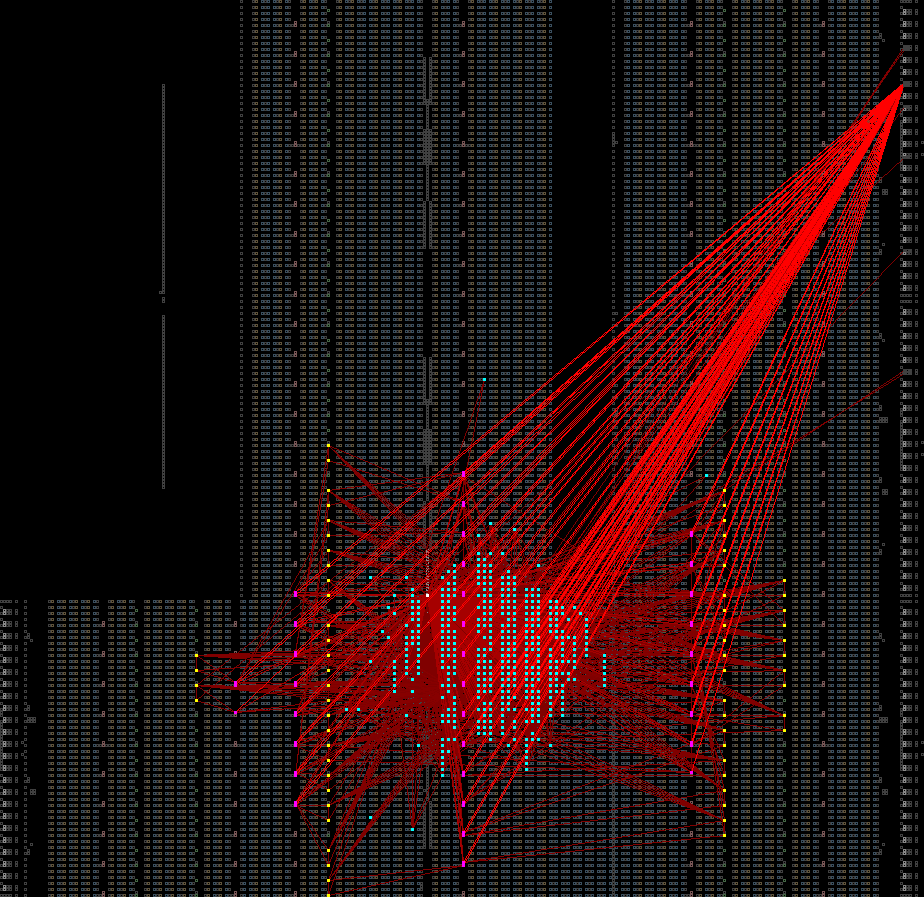
\includegraphics[valign=t, scale=0.25]{figures/results/PlacerGreedyRandom/00000299.png}
    \captionof{figure}{Snapshots of placement of a 2048th order FIR Filter on a xc7z020 FPGA. \textbf{From left to right:} \textbf{(1)} Initial random placement, \textbf{(2)} After 10 passes, \textbf{(3)} After 100 passes, \textbf{(4)} Final placement after 300 passes.}
    \label{fig:PGRSnapshots}
}
{
    \centering
    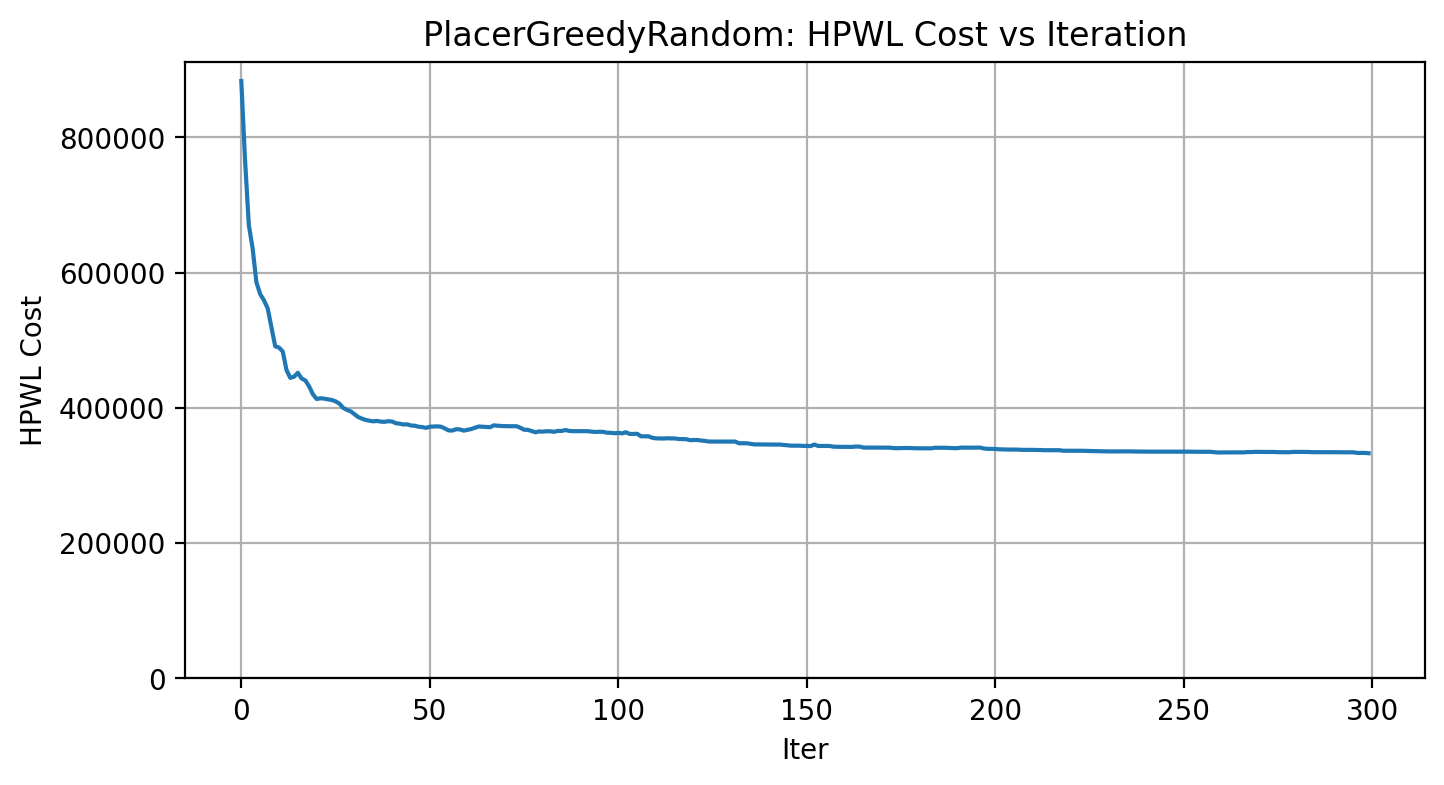
\includegraphics[width=0.7\columnwidth]{figures/results/PlacerGreedyRandom/PlacerGreedyRandom_cost_history.png}
    \captionof{figure}{Total HPWL Cost vs number of passes. Final cost: 333013.}
    \label{fig:PGRCurve}
}

\subsection{Greedy Algorithm (Directed/Midpoint Moves)}
{
    \centering
    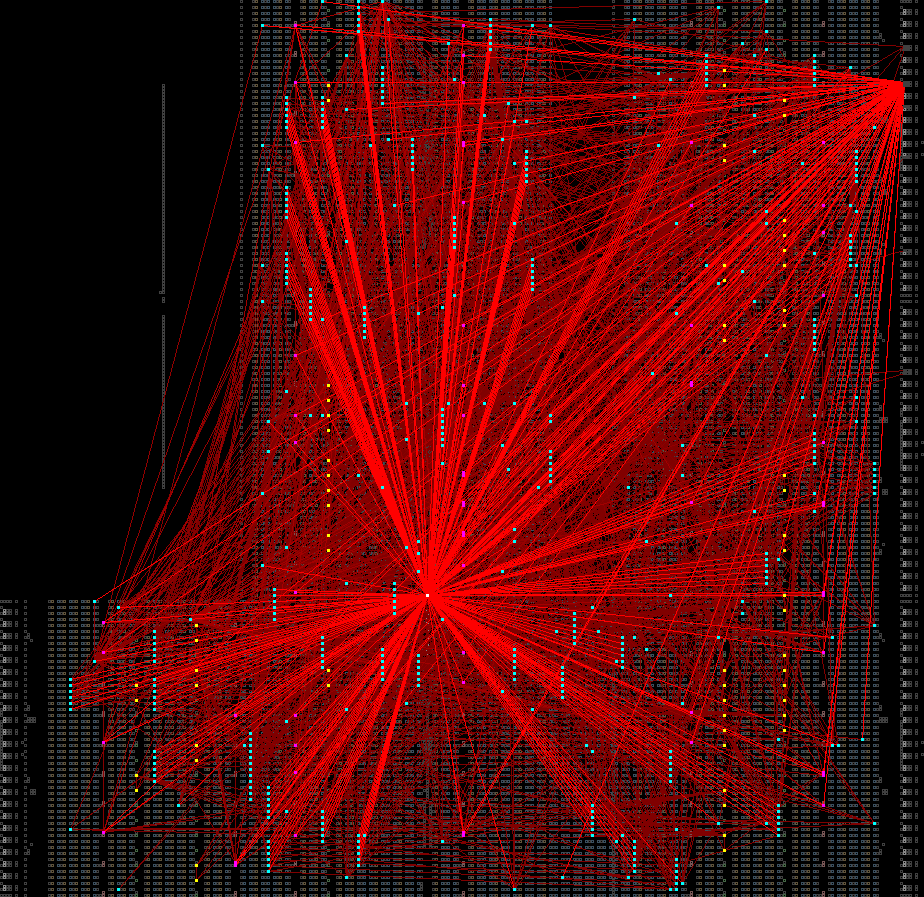
\includegraphics[valign=t, scale=0.25]{figures/results/PlacerGreedyMidpoint/random_placement.png}
    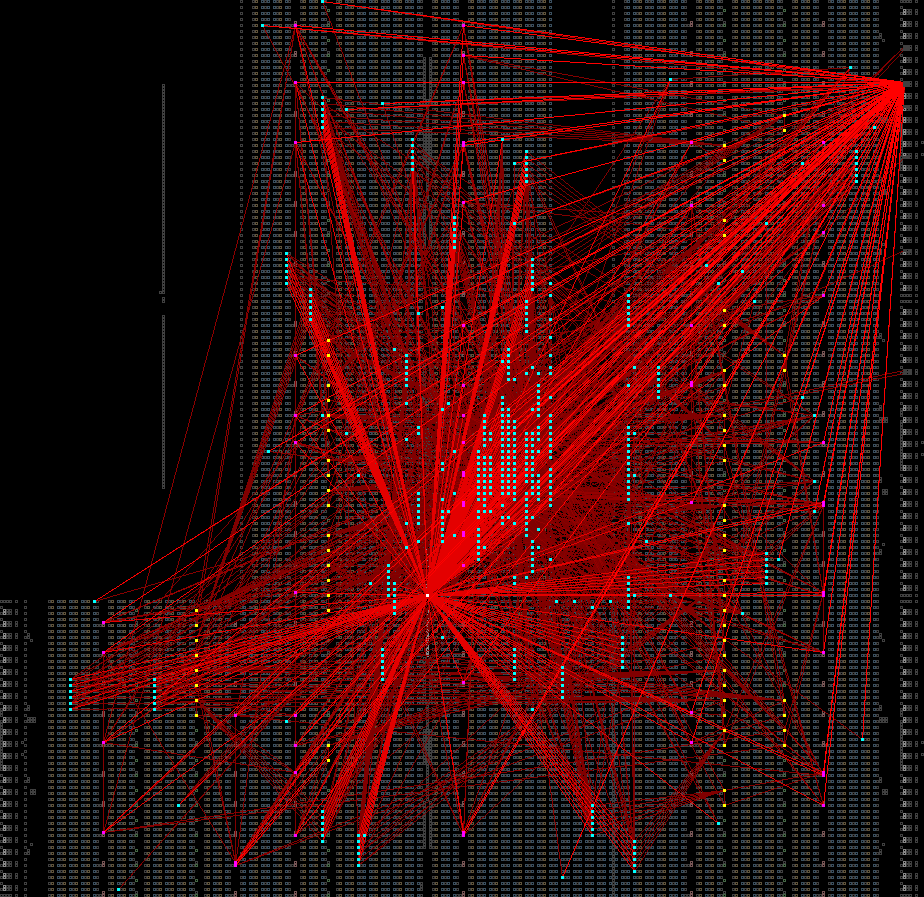
\includegraphics[valign=t, scale=0.25]{figures/results/PlacerGreedyMidpoint/00000010.png}
    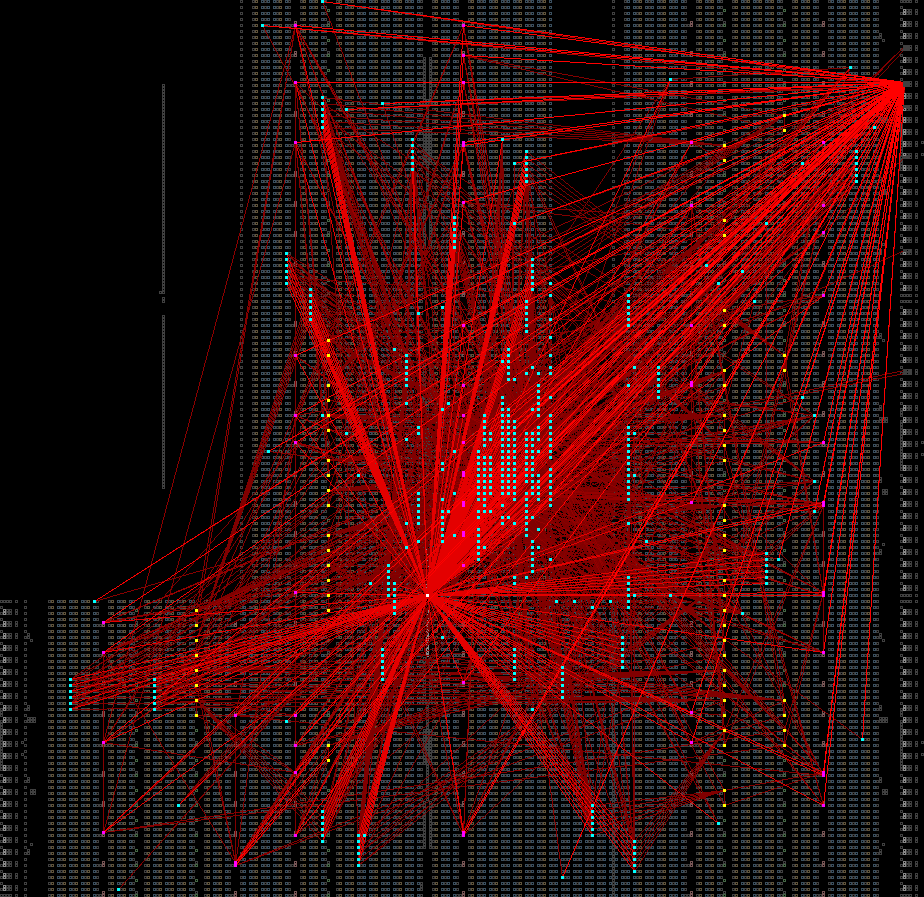
\includegraphics[valign=t, scale=0.25]{figures/results/PlacerGreedyMidpoint/00000100.png}
    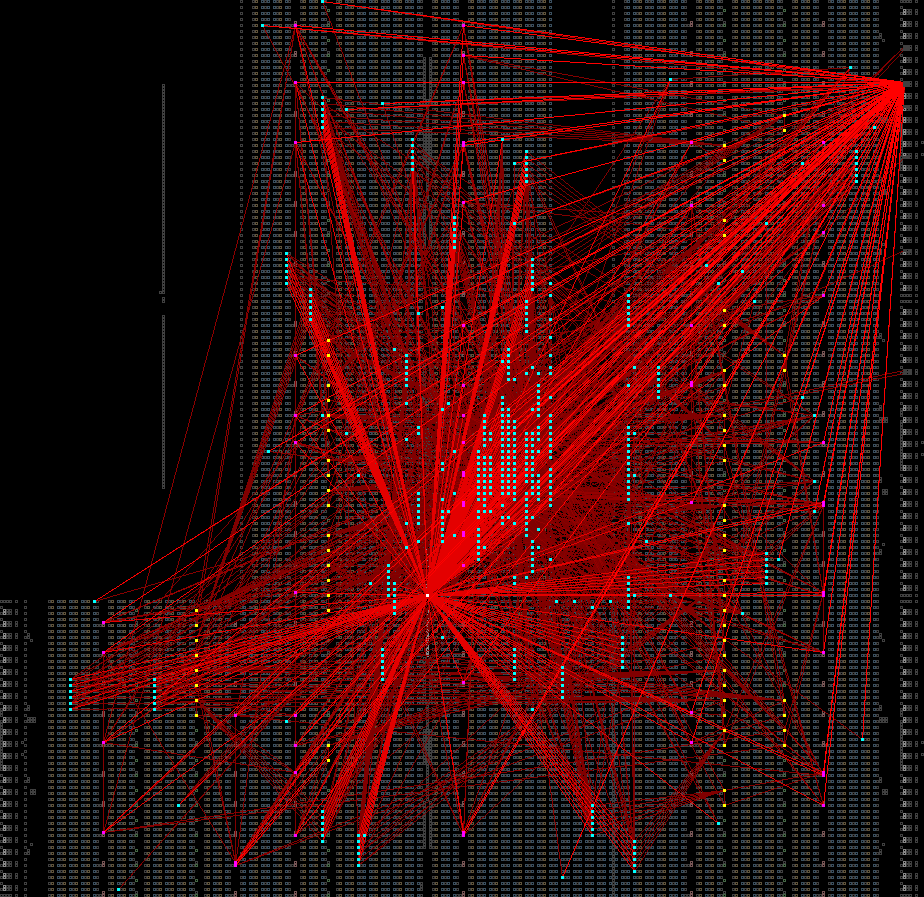
\includegraphics[valign=t, scale=0.25]{figures/results/PlacerGreedyMidpoint/00000299.png}
    \captionof{figure}{Snapshots of placement of a 2048th order FIR Filter on a xc7z020 FPGA. \textbf{From left to right:} \textbf{(1)} Initial random placement, \textbf{(2)} After 10 passes, \textbf{(3)} After 100 passes, \textbf{(4)} Final placement after 300 passes.}
    \label{fig:PGMSnapshots}
}
{
    \centering
    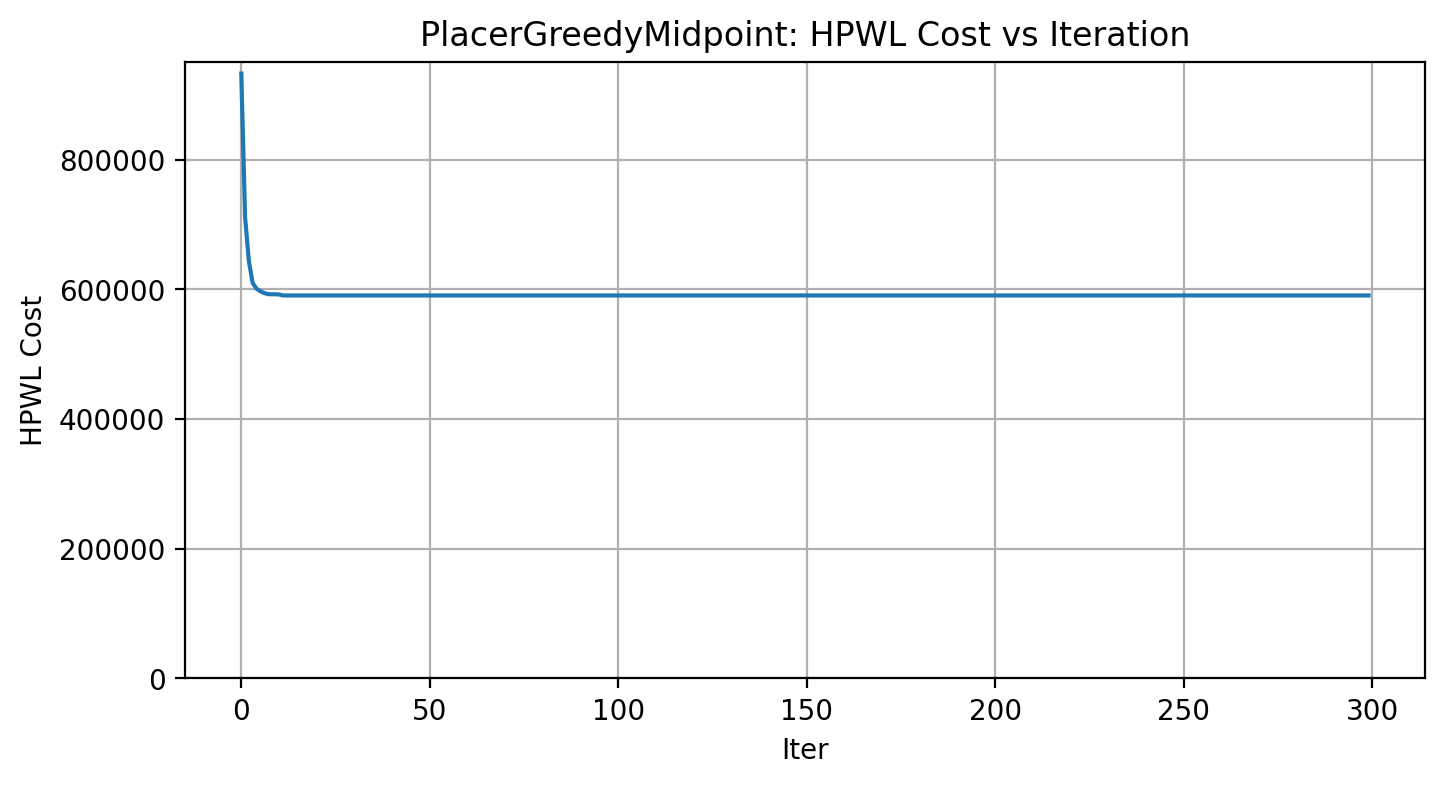
\includegraphics[width=0.7\columnwidth]{figures/results/PlacerGreedyMidpoint/PlacerGreedyMidpoint_cost_history.png}
    \captionof{figure}{Total HPWL Cost vs number of passes. Final cost: 590578.}
    \label{fig:PGMCurve}
}

\subsection{Simulated Annealing (Undirected/Random Moves)}
{
    \centering
    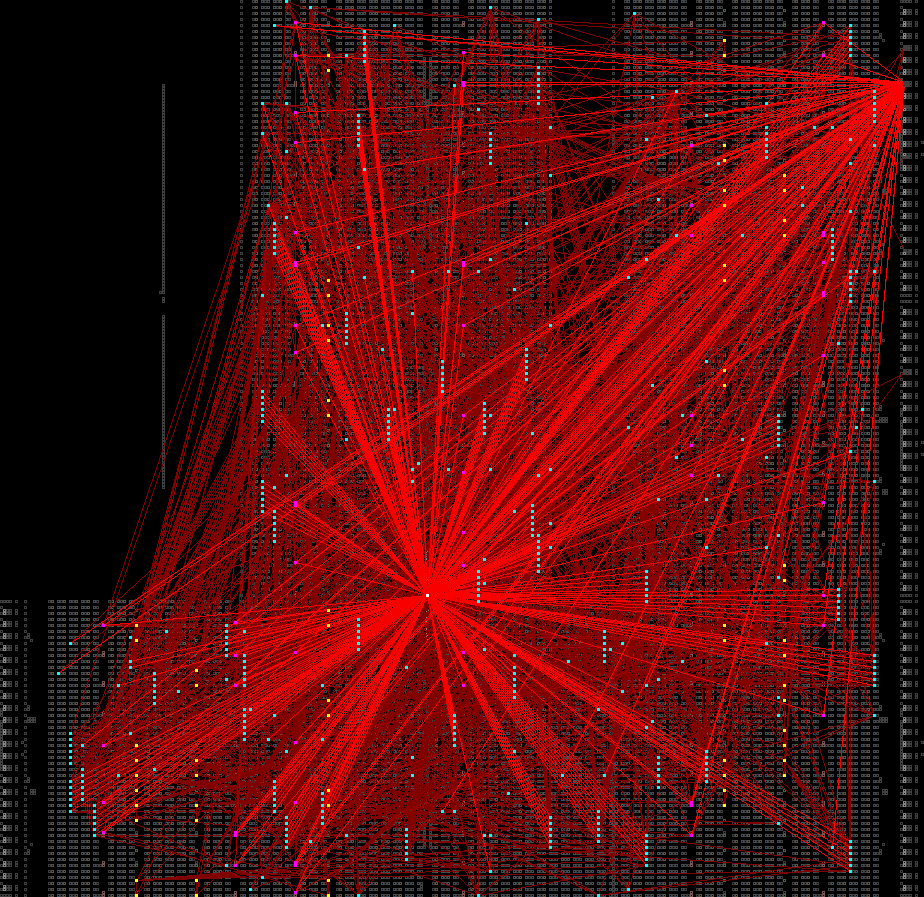
\includegraphics[valign=t, scale=0.25]{figures/results/PlacerAnnealRandom/random_placement.png}
    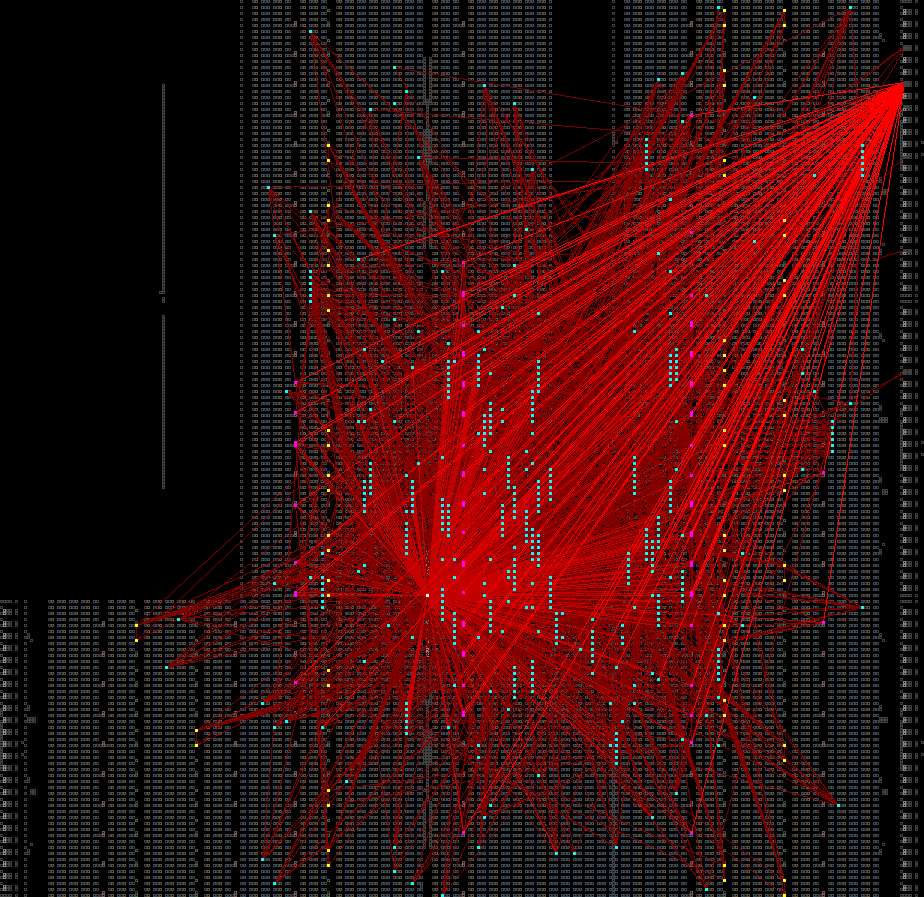
\includegraphics[valign=t, scale=0.25]{figures/results/PlacerAnnealRandom/00000010.png}
    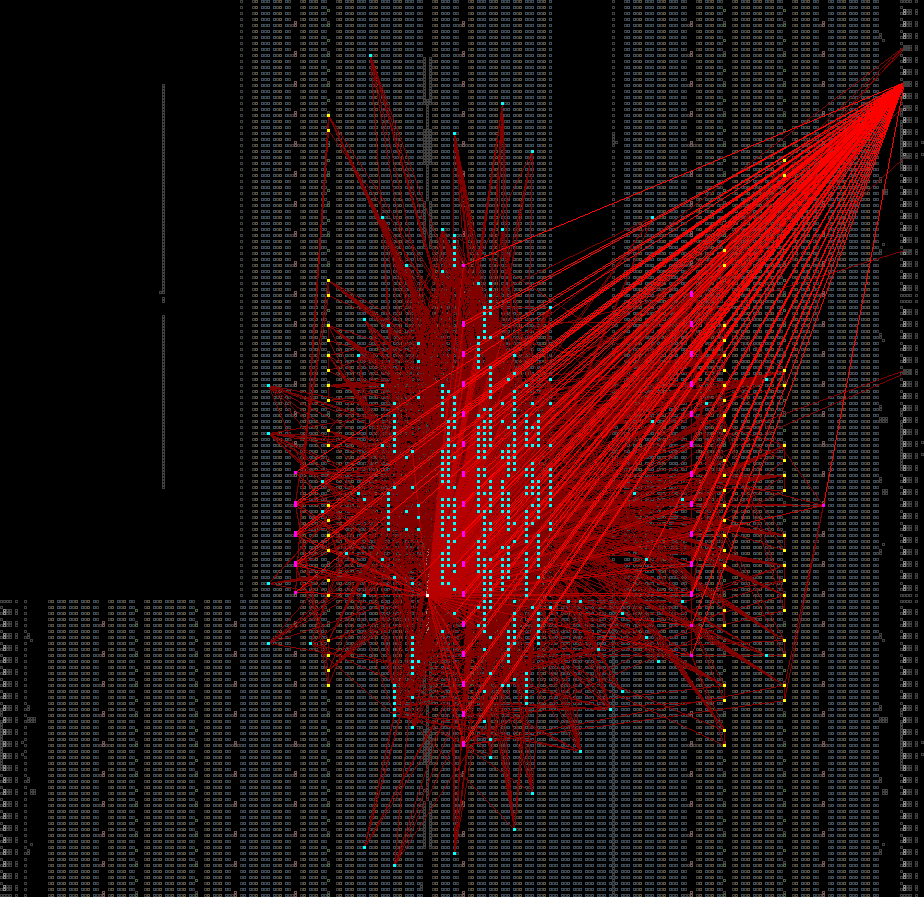
\includegraphics[valign=t, scale=0.25]{figures/results/PlacerAnnealRandom/00000100.png}
    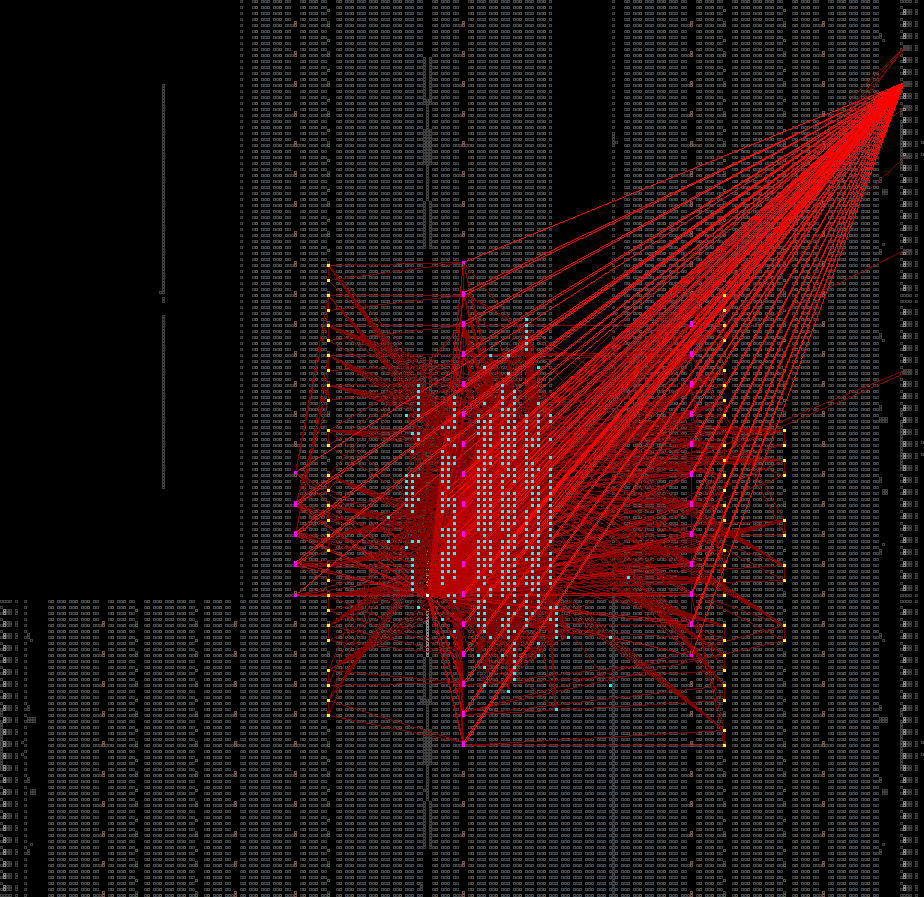
\includegraphics[valign=t, scale=0.25]{figures/results/PlacerAnnealRandom/00000299.png}
    \captionof{figure}{Snapshots of placement of a 2048th order FIR Filter on a xc7z020 FPGA. \textbf{From left to right:} \textbf{(1)} Initial random placement, \textbf{(2)} After 10 passes, \textbf{(3)} After 100 passes, \textbf{(4)} Final placement after 300 passes.}
    \label{fig:PARSnapshots}
}
{
    \centering
    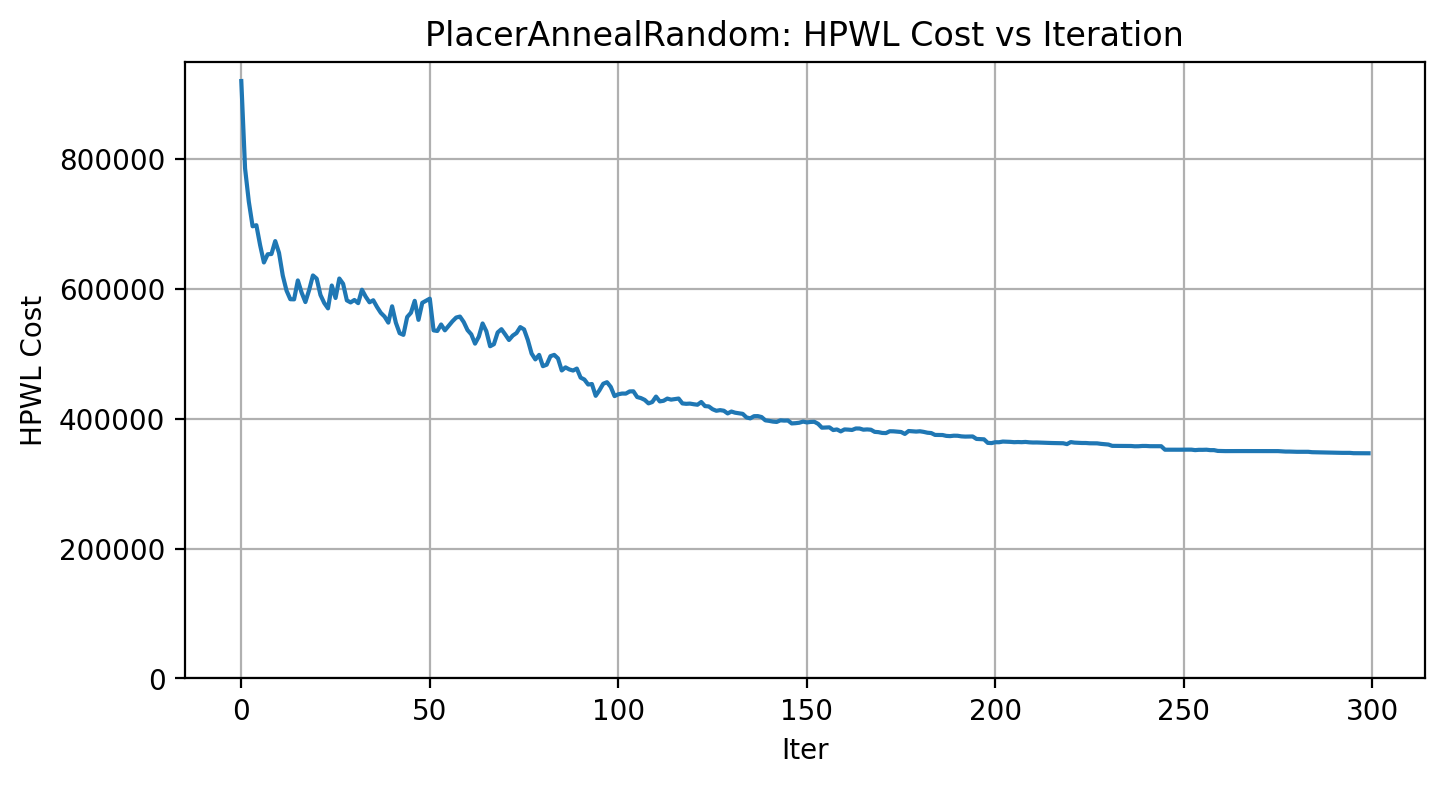
\includegraphics[width=0.7\columnwidth]{figures/results/PlacerAnnealRandom/PlacerAnnealRandom_cost_history.png}
    \captionof{figure}{Total HPWL Cost vs number of passes. Final cost: 346676.}
    \label{fig:PARCurve}
}

\subsection{Simulated Annealing (Directed/Midpoint Moves)}
{
    \centering
    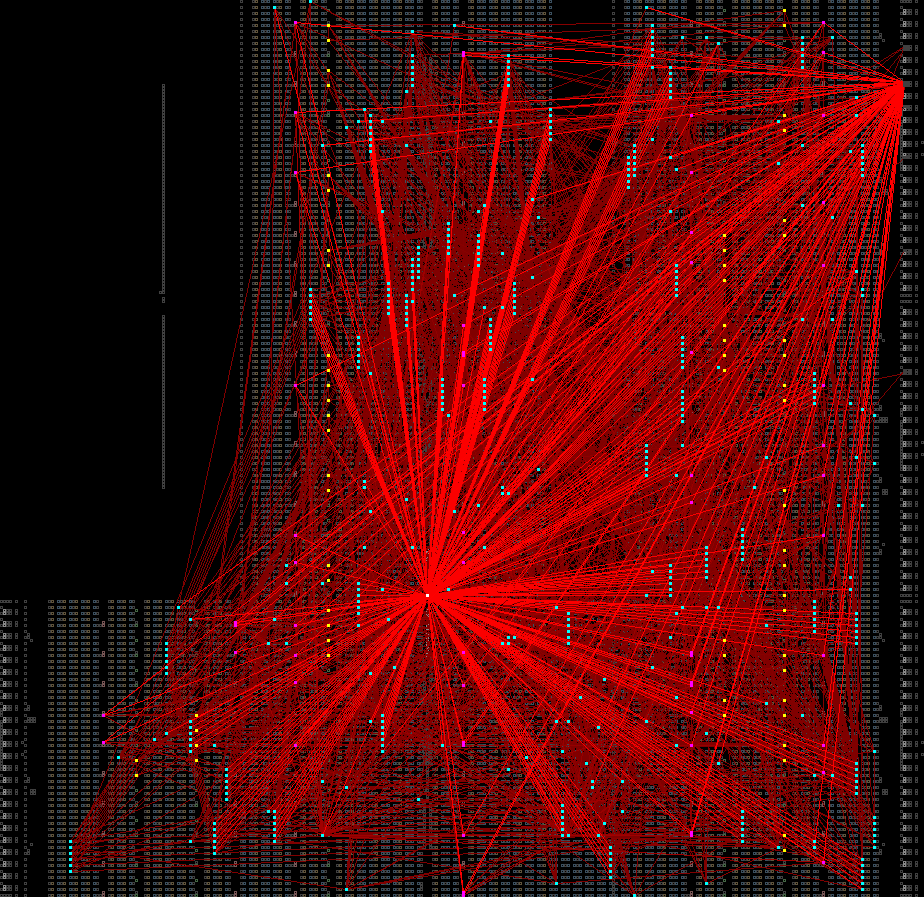
\includegraphics[valign=t, scale=0.25]{figures/results/PlacerAnnealMidpoint/random_placement.png}
    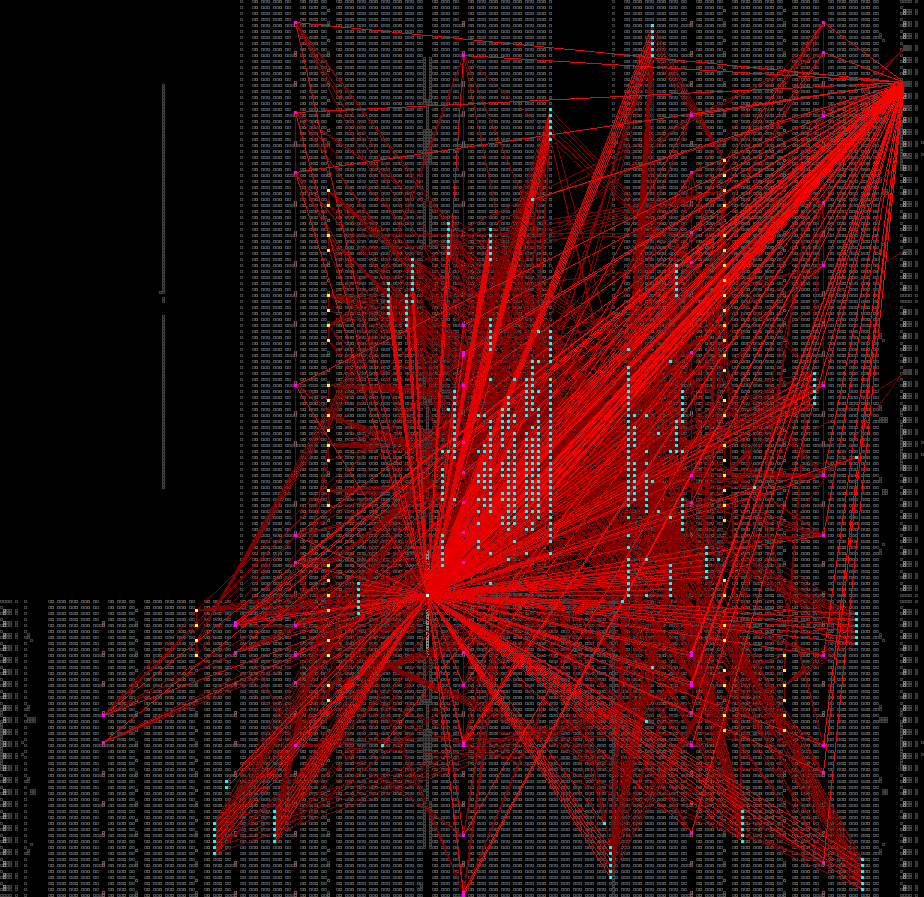
\includegraphics[valign=t, scale=0.25]{figures/results/PlacerAnnealMidpoint/00000010.png}
    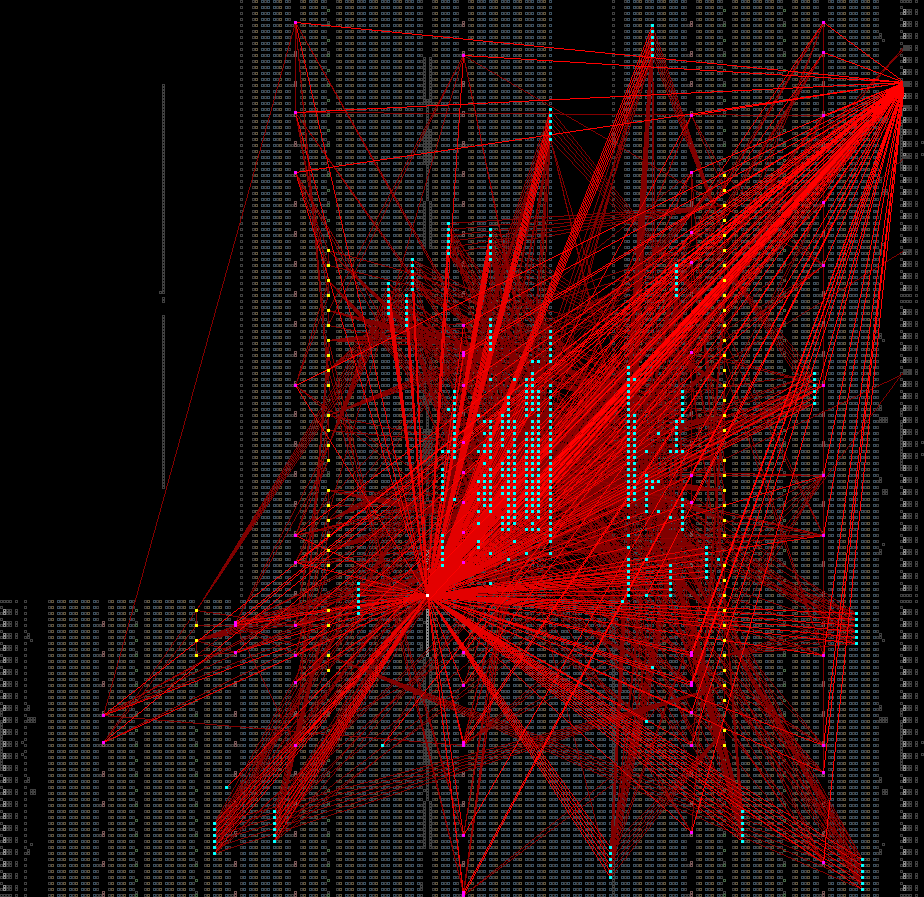
\includegraphics[valign=t, scale=0.25]{figures/results/PlacerAnnealMidpoint/00000100.png}
    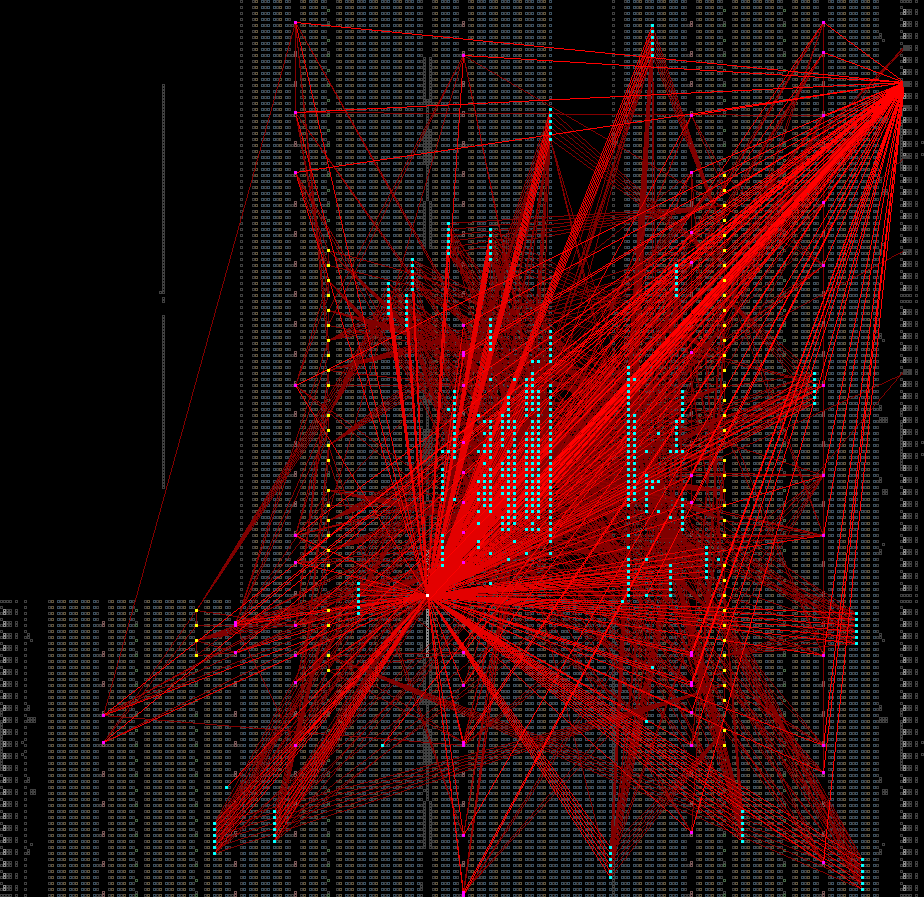
\includegraphics[valign=t, scale=0.25]{figures/results/PlacerAnnealMidpoint/00000299.png}
    \captionof{figure}{Snapshots of placement of a 2048th order FIR Filter on a xc7z020 FPGA. \textbf{From left to right:} \textbf{(1)} Initial random placement, \textbf{(2)} After 10 passes, \textbf{(3)} After 100 passes, \textbf{(4)} Final placement after 300 passes.}
    \label{fig:PAMSnapshots}
}
{
    \centering
    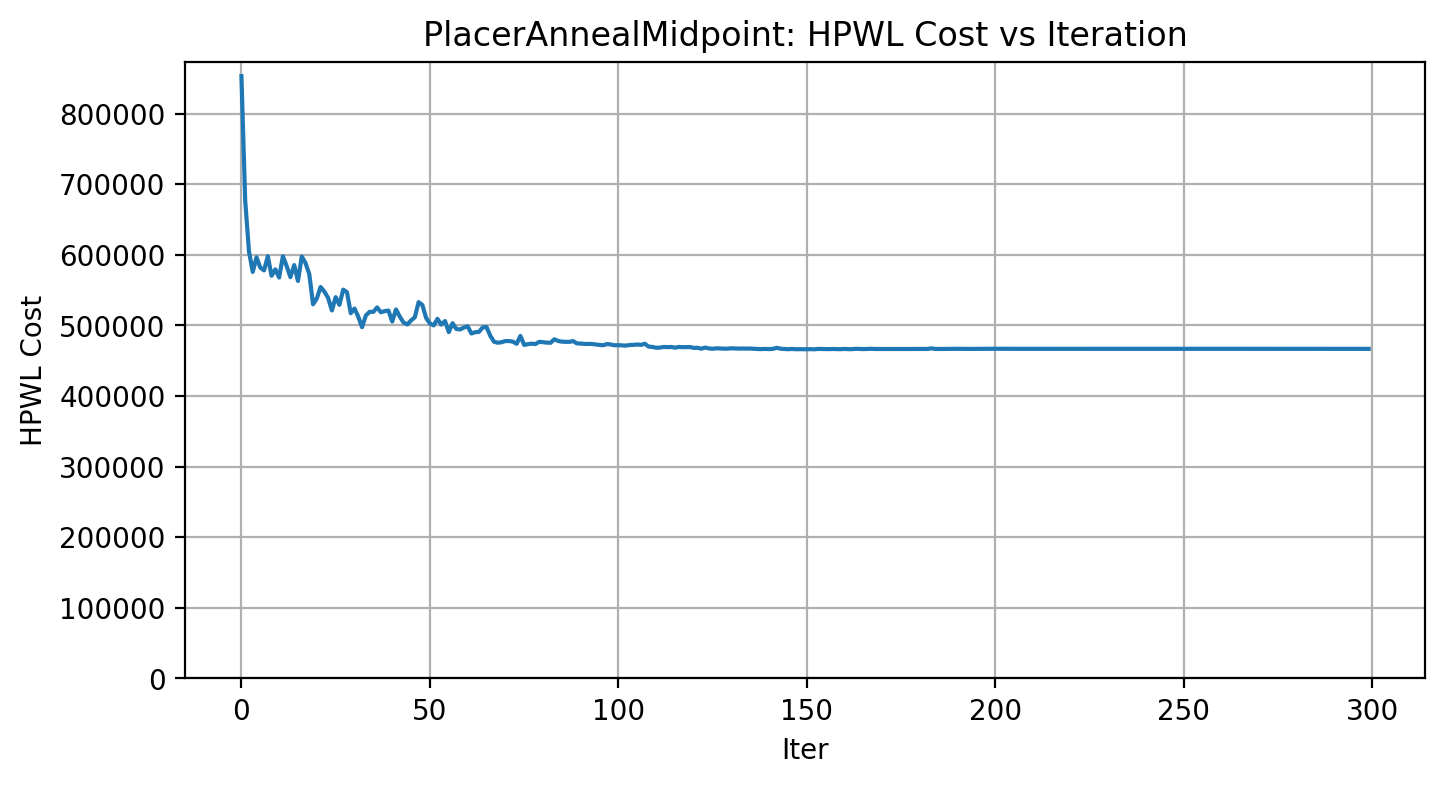
\includegraphics[width=0.7\columnwidth]{figures/results/PlacerAnnealMidpoint/PlacerAnnealMidpoint_cost_history.png}
    \captionof{figure}{Total HPWL Cost vs number of passes. Final cost: 466855.}
    \label{fig:PAMCurve}
}

\subsection{Simulated Annealing (Hybrid: Random + Midpoint)}
{
    \centering
    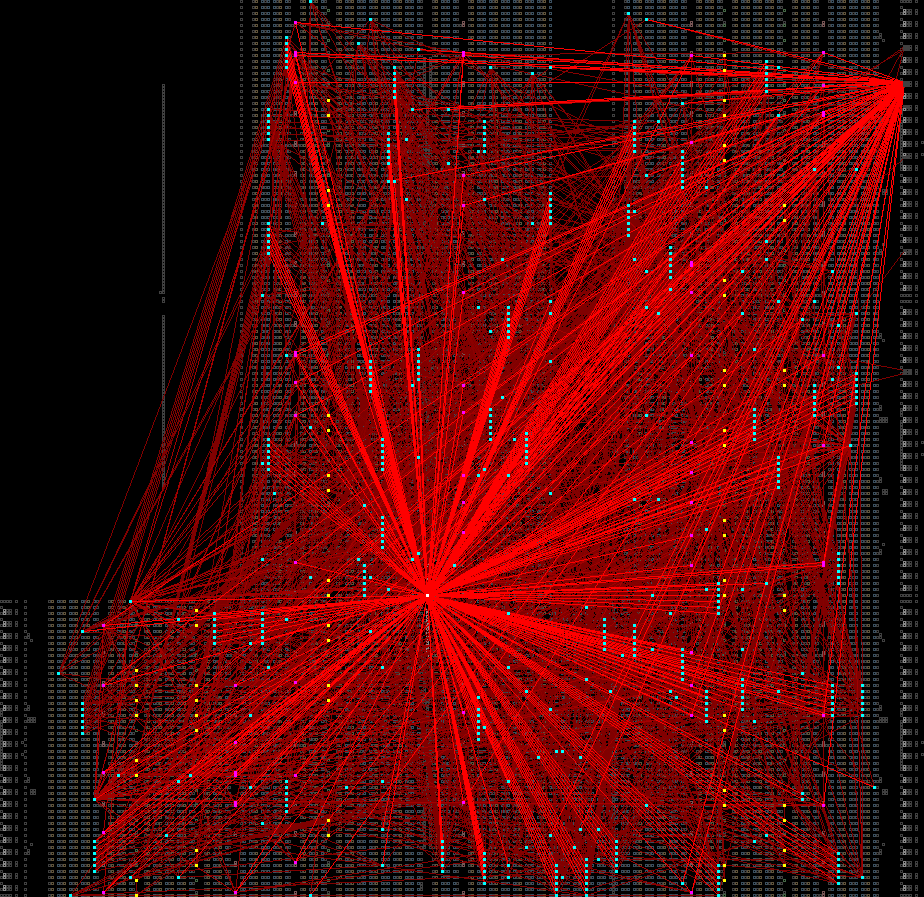
\includegraphics[valign=t, scale=0.25]{figures/results/PlacerAnnealHybrid/random_placement.png}
    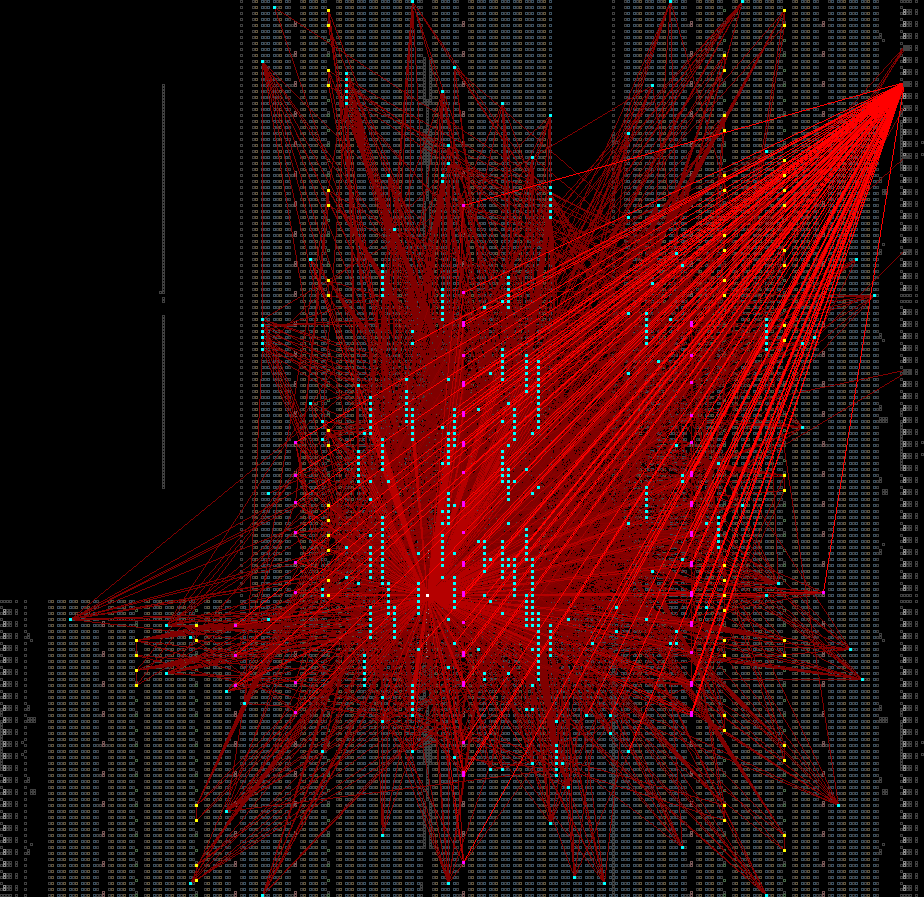
\includegraphics[valign=t, scale=0.25]{figures/results/PlacerAnnealHybrid/00000010.png}
    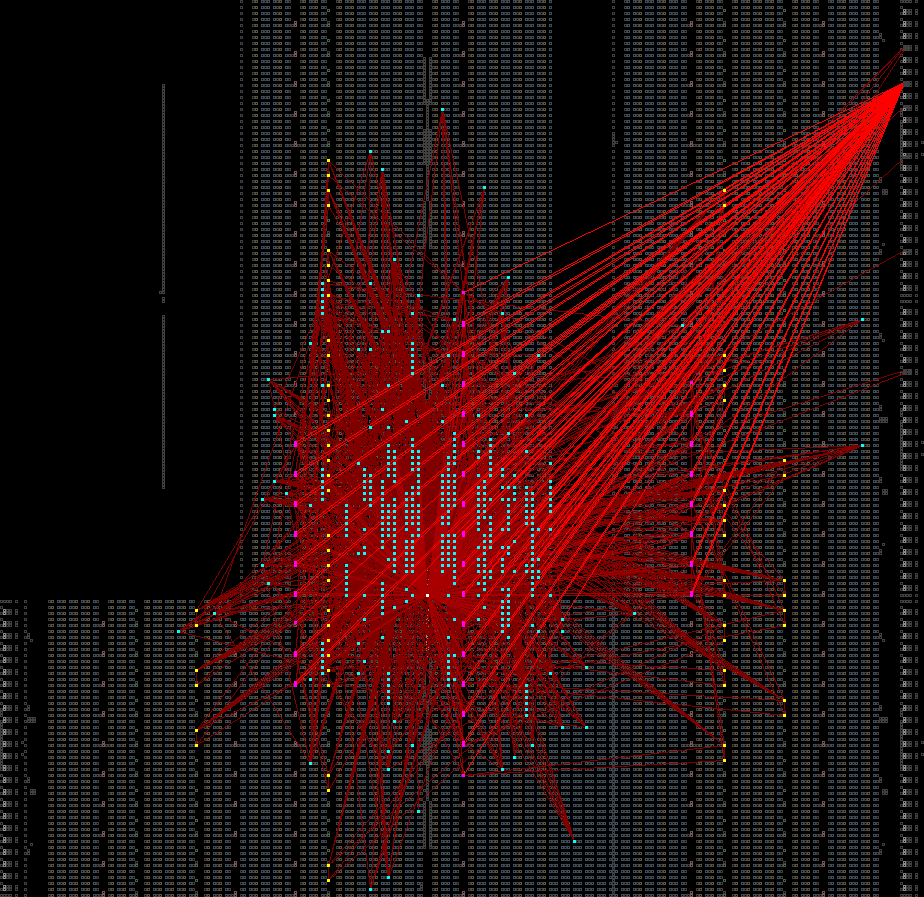
\includegraphics[valign=t, scale=0.25]{figures/results/PlacerAnnealHybrid/00000100.png}
    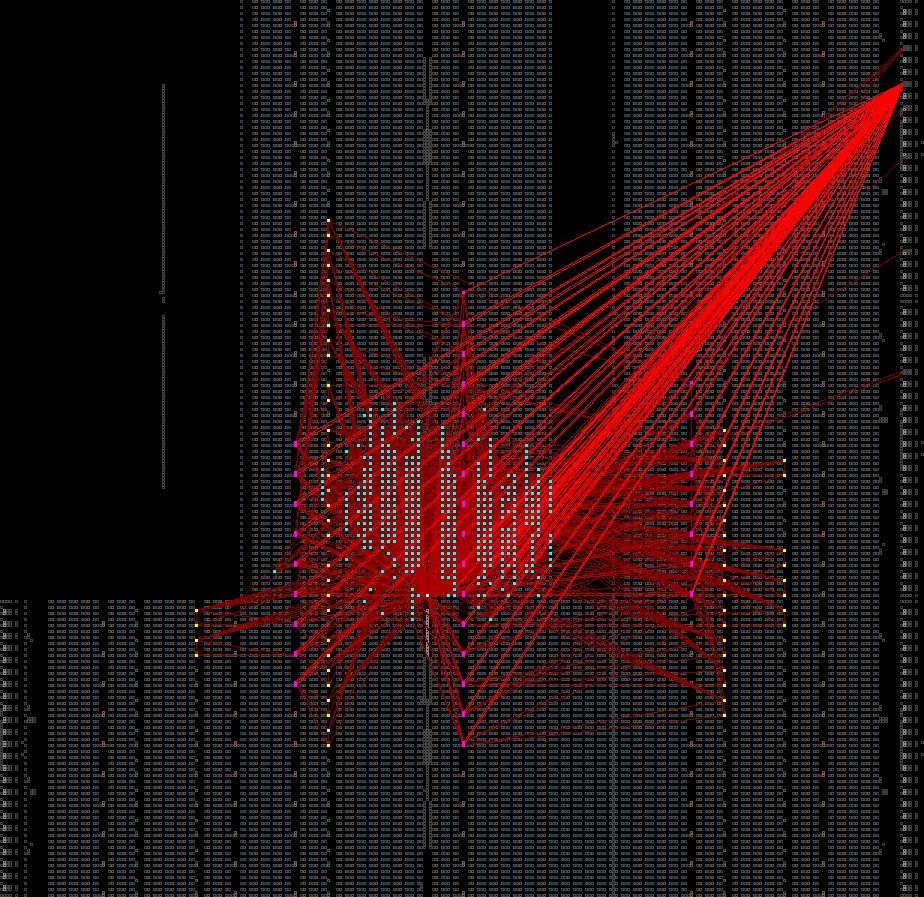
\includegraphics[valign=t, scale=0.25]{figures/results/PlacerAnnealHybrid/00000299.png}
    \captionof{figure}{Snapshots of placement of a 2048th order FIR Filter on a xc7z020 FPGA. \textbf{From left to right:} \textbf{(1)} Initial random placement, \textbf{(2)} After 10 passes, \textbf{(3)} After 100 passes, \textbf{(4)} Final placement after 300 passes.}
    \label{fig:PAHSnapshots}
}
{
    \centering
    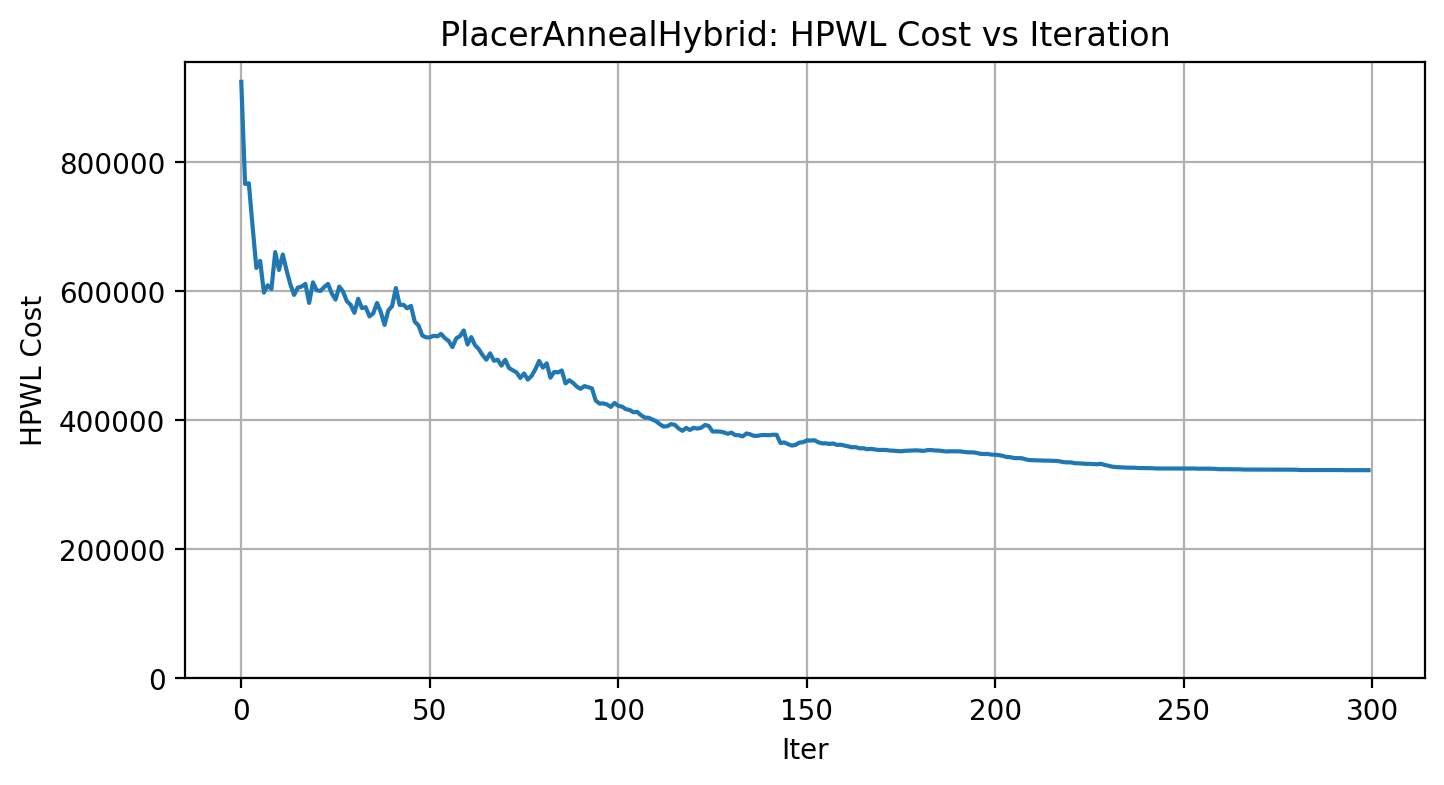
\includegraphics[width=0.7\columnwidth]{figures/results/PlacerAnnealHybrid/PlacerAnnealHybrid_cost_history.png}
    \captionof{figure}{Total HPWL Cost vs number of passes. Final cost: 322933.}
    \label{fig:PAHCurve}
}


\begin{multicols}{2}
